% Gabarit pandoc des corrigés publiés (brut et guidé). Contenu sans marque ni nom de site.
% Compilation : lualatex (latexmk -lualatex).
% Le Markdown reste la source unique : ne pas éditer ce fichier .tex à la main.
\documentclass[11pt,a4paper]{article}

% --- Moteur, polices (Latin Modern) et langue ---------------------------------
\usepackage{iftex}
\ifLuaTeX\else\errmessage{Ce document se compile avec lualatex}\fi
\usepackage{amsmath,amssymb,mathtools}
\usepackage{fontspec}
% mathrm=sym : \mathrm prend ses glyphes dans la police mathématique (ℓ, μ, Ω), comme KaTeX.
\usepackage[math-style=TeX,bold-style=TeX,mathrm=sym]{unicode-math}
% Repli pour les glyphes absents de Latin Modern (indices et exposants Unicode,
% flèches, filets des schémas en texte, symboles) : DejaVu, puis Latin Modern Math
% (ℓ, lettres mathématiques Unicode des légendes).
\directlua{
  luaotfload.add_fallback("repliTexte", {"DejaVuSerif:mode=harf;", "DejaVuSans:mode=harf;", "file:latinmodern-math.otf:mode=harf;"})
  luaotfload.add_fallback("repliMono", {"DejaVuSansMono:mode=harf;", "DejaVuSans:mode=harf;", "file:latinmodern-math.otf:mode=harf;"})
}
\setmainfont{Latin Modern Roman}[RawFeature={fallback=repliTexte}]
\setsansfont{Latin Modern Sans}[RawFeature={fallback=repliTexte}]
\setmonofont{Latin Modern Mono}[RawFeature={fallback=repliMono}]
\setmathfont{Latin Modern Math}
\usepackage[french]{babel}
\frenchsetup{SmallCapsFigTabCaptions=false}

% --- Mise en page --------------------------------------------------------------
\usepackage[a4paper,margin=2.2cm,headheight=14pt,footskip=1.2cm]{geometry}
\usepackage{microtype}
\setlength{\emergencystretch}{4em}
\tolerance=1500
\setlength{\parindent}{0pt}
\setlength{\parskip}{0.55\baselineskip plus 2pt minus 1pt}
\usepackage{xcolor}
% Gris nommés : babel-french rend « ! » actif dans le document.
\definecolor{gris2}{gray}{0.98}
\definecolor{gris3}{gray}{0.97}
\definecolor{gris5}{gray}{0.95}
\definecolor{gris35}{gray}{0.65}
\definecolor{gris40}{gray}{0.60}
\definecolor{gris45}{gray}{0.55}
\definecolor{gris50}{gray}{0.50}
\definecolor{gris55}{gray}{0.45}
\definecolor{gris60}{gray}{0.40}
\definecolor{gris65}{gray}{0.35}
\definecolor{gris70}{gray}{0.30}
\definecolor{gris80}{gray}{0.20}
\definecolor{gris85}{gray}{0.15}
\usepackage{graphicx}
\usepackage{float}
\usepackage{caption}
\captionsetup{font=small,labelformat=empty,justification=centering}
\usepackage{booktabs,longtable,array,multirow,calc}
\usepackage{siunitx}
\sisetup{locale=FR}
\usepackage[version=4]{mhchem}
\usepackage{listings}
\usepackage{fancyhdr}
\usepackage{lastpage}
\usepackage[most]{tcolorbox}
\usepackage{enumitem}
\setlist{nosep,leftmargin=*,topsep=2pt}
\usepackage[hidelinks,unicode]{hyperref}
\usepackage{bookmark}
\hypersetup{pdftitle={CCINP TPC — Modélisation de systèmes physiques ou chimiques 2026},pdfauthor={Rédigé par IA},pdfcreator={LaTeX},pdfsubject={Corrigé brut}}
\usepackage{xurl}

% --- Pandoc : listes, tableaux, figures ----------------------------------------
\providecommand{\passthrough}[1]{#1}
\providecommand{\tightlist}{\setlength{\itemsep}{0pt}\setlength{\parskip}{0pt}}

\makeatletter
\def\maxwidth{\ifdim\Gin@nat@width>\linewidth\linewidth\else\Gin@nat@width\fi}
\def\maxheight{\ifdim\Gin@nat@height>0.55\textheight 0.55\textheight\else\Gin@nat@height\fi}
\makeatother
\setkeys{Gin}{width=\maxwidth,height=\maxheight,keepaspectratio}
\setcounter{secnumdepth}{-\maxdimen}
\providecommand{\pandocbounded}[1]{#1}

% --- Code (listings) -----------------------------------------------------------
\lstset{
  basicstyle=\ttfamily\small,
  columns=fullflexible,
  keepspaces=true,
  breaklines=true,
  breakatwhitespace=false,
  postbreak=\mbox{\textcolor{gris50}{$\hookrightarrow$}\space},
  frame=single,
  rulecolor=\color{gris35},
  framesep=4pt,
  xleftmargin=5pt,xrightmargin=5pt,
  backgroundcolor=\color{gris3},
  keywordstyle=\bfseries,
  commentstyle=\color{gris65},
  stringstyle=\color{gris80},
  showstringspaces=false,
  tabsize=4,
  extendedchars=true,
  aboveskip=6pt,belowskip=6pt,
}

% --- Macros des corrigés (KaTeX ↔ LaTeX) ---------------------------------------
% Les corrigés sont écrits pour KaTeX : on définit ici ce que KaTeX connaît et
% que LaTeX n'a pas, sans jamais retoucher le Markdown.
\providecommand{\R}{\mathbb{R}}
\providecommand{\N}{\mathbb{N}}
\providecommand{\Z}{\mathbb{Z}}
\providecommand{\Q}{\mathbb{Q}}
\providecommand{\C}{\mathbb{C}}
\providecommand{\dd}{\mathrm{d}}
\providecommand{\llbracket}{\lBrack}
\providecommand{\rrbracket}{\rBrack}
\providecommand{\lBrace}{\lbrace}
\providecommand{\rBrace}{\rbrace}
\providecommand{\Box}{\square}
\providecommand{\Diamond}{\lozenge}
\providecommand{\varnothing}{\emptyset}
\providecommand{\argmax}{\operatorname*{arg\,max}}
\providecommand{\argmin}{\operatorname*{arg\,min}}
\renewcommand{\leq}{\leqslant}
\renewcommand{\geq}{\geqslant}

% Équation hors texte : réduite à la largeur de la ligne si elle déborde.
\newsavebox{\boiteequation}
\newcommand{\equationajustee}[1]{%
  \sbox{\boiteequation}{$\displaystyle #1$}%
  \ifdim\wd\boiteequation>\linewidth
    \[\resizebox{\linewidth}{!}{\usebox{\boiteequation}}\]%
  \else
    \[#1\]%
  \fi}

% --- Encadrés pédagogiques (sobres, lisibles en noir et blanc) -----------------
\tcbset{
  encadre/.style={
    enhanced,breakable,sharp corners,
    colback=white,colframe=gris55,
    boxrule=0.4pt,leftrule=2.2pt,
    left=6pt,right=6pt,top=3pt,bottom=3pt,
    before skip=6pt,after skip=6pt,
    fonttitle=\bfseries\small,coltitle=black,
    attach title to upper,after title={\quad},
    parbox=false,
  }
}
\newtcolorbox{indication}[1]{encadre,colframe=gris45,colback=gris2,title={Indication~#1}}
\newtcolorbox{methode}{encadre,colframe=gris70,title={Méthode}}
\newtcolorbox{piege}{encadre,colframe=gris85,boxrule=0.8pt,leftrule=2.2pt,title={Piège}}
\newtcolorbox{jury}{encadre,colframe=gris60,colback=gris5,title={Jury}}
\newtcolorbox{encadrenote}{encadre,colframe=gris40}

% --- Titres de section ---------------------------------------------------------
\usepackage{titlesec}
\titleformat{\section}{\Large\bfseries}{}{0pt}{}
\titleformat{\subsection}{\large\bfseries}{}{0pt}{}
\titleformat{\subsubsection}{\normalsize\bfseries}{}{0pt}{}
\titlespacing*{\section}{0pt}{14pt plus 4pt minus 2pt}{6pt}
\titlespacing*{\subsection}{0pt}{10pt plus 3pt minus 2pt}{4pt}
\titlespacing*{\subsubsection}{0pt}{8pt plus 2pt minus 2pt}{2pt}

% --- En-tête et pied de page ---------------------------------------------------
\pagestyle{fancy}
\fancyhf{}
\fancyhead[L]{\small\textsc{Corrigé brut} · CCINP TPC}
\fancyhead[R]{\small Modélisation de systèmes physiques ou chimiques 2026}
\fancyfoot[L]{\footnotesize Corrigé rédigé par IA, non officiel}
\fancyfoot[R]{\footnotesize \thepage\,/\,\pageref*{LastPage}}
\renewcommand{\headrulewidth}{0.4pt}
\renewcommand{\footrulewidth}{0pt}
\fancypagestyle{plain}{\fancyhf{}\fancyfoot[R]{\footnotesize \thepage\,/\,\pageref*{LastPage}}\fancyfoot[L]{\footnotesize Corrigé rédigé par IA, non officiel}\renewcommand{\headrulewidth}{0pt}}

\begin{document}
\thispagestyle{plain}
\begin{center}
  {\small\scshape Corrigé brut}\par\smallskip
  {\LARGE\bfseries CCINP TPC — Modélisation de systèmes physiques ou chimiques 2026\par}\medskip
  {\large CCINP · TPC · Modélisation de systèmes physiques ou chimiques · 2026\par}
\end{center}
\vspace{2pt}\hrule\vspace{8pt}

\emph{Corrigé rédigé par IA, non officiel. Signalez toute erreur.}

Épreuve TPC7MO, durée 4 h, calculatrice interdite. \emph{Étude d'un spectrophotomètre infrarouge.}

\hypertarget{partie-i-absorption-vibrationnelle}{%
\section{Partie I --- Absorption vibrationnelle}\label{partie-i-absorption-vibrationnelle}}

\hypertarget{i.1-moduxe8le-classique-de-la-vibration-dune-moluxe9cule-diatomique}{%
\subsection{I.1 --- Modèle classique de la vibration d'une molécule diatomique}\label{i.1-moduxe8le-classique-de-la-vibration-dune-moluxe9cule-diatomique}}

\hypertarget{q1}{%
\subsubsection{Q1}\label{q1}}

L'argument d'une exponentielle est sans dimension : \(\alpha(x - x_e)\) est sans dimension.

Comme \(x\) est une longueur et que l'on retranche \(x_e\) à \(x\), \(x_e\) est une longueur. Donc \(\alpha\) est l'inverse d'une longueur.

Enfin \(\bigl(1 - {\mathrm{e}}^{-\alpha(x-x_e)}\bigr)^2\) est sans dimension et \(E_p\) est une énergie, donc \(D\) est une énergie.

\equationajustee{\boxed{\begin{aligned}{}&D\ \text{en J}\ (\mathrm{kg\,m^2\,s^{-2}}) \\
&\alpha\ \text{en}\ \mathrm{m^{-1}} \\
&x_e\ \text{en m}
\end{aligned}}}

\hypertarget{q2}{%
\subsubsection{Q2}\label{q2}}

Allure de la courbe (figure 1) : branche répulsive très raide aux petits \(x\), minimum nul en \(x = x_e\), puis croissance avec un point d'inflexion vers l'asymptote horizontale \(E_p = D\).

\begin{figure}[H]
\centering
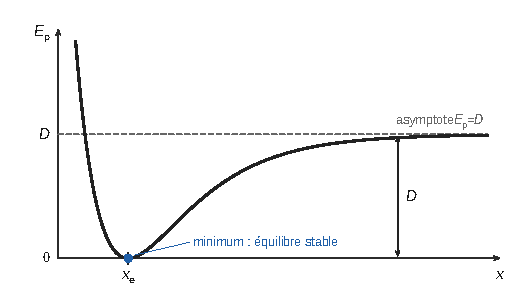
\includegraphics{figures/q02-potentiel-morse.pdf}
\caption*{Figure 1 --- Potentiel de Morse, minimum nul en x\_e (équilibre stable)
et asymptote E\_p = D, D profondeur du puits}
\end{figure}

En effet \(E_p = D(1-u)^2 \ge 0\) avec \(u = {\mathrm{e}}^{-\alpha(x - x_e)}\), et \(E_p = 0 \iff u = 1 \iff x = x_e\).

La position d'équilibre est \(x = x_e\) (où \(\mathrm{d}E_p/\mathrm{d}x = 0\)). \textbf{Cet équilibre est stable car \(E_p\) y présente un minimum} : tout écart fait apparaître une force \(-\mathrm{d}E_p/\mathrm{d}x\) qui ramène le système vers \(x_e\).

\hypertarget{q3}{%
\subsubsection{Q3}\label{q3}}

\(\alpha > 0\) donc \({\mathrm{e}}^{-\alpha(x - x_e)} \to 0\) quand \(x \to +\infty\), et \(E_p \to D\). Comme \(E_p(x_e) = 0\),

\equationajustee{\boxed{D = \lim_{x\to+\infty} E_p(x) - E_p(x_e)}}

Sur l'axe des ordonnées, \(D\) est l'ordonnée de l'asymptote horizontale (comptée depuis le fond du puits, d'ordonnée nulle) : c'est la profondeur du puits, énergie à fournir pour dissocier la molécule au repos en \(x_e\).

\hypertarget{q4}{%
\subsubsection{Q4}\label{q4}}

Posons \(u = {\mathrm{e}}^{-\alpha(x - x_e)}\), donc \(u' = -\alpha u\) et \(E_p = D(1-u)^2\).

\equationajustee{\frac{\mathrm{d}E_p}{\mathrm{d}x} = 2D(1-u)(-u') = \boxed{2\alpha D\,{\mathrm{e}}^{-\alpha(x - x_e)}\left(1 - {\mathrm{e}}^{-\alpha(x - x_e)}\right)}}

En dérivant \(2\alpha D(u - u^2)\) :

\equationajustee{\frac{{\mathrm{d}}^2E_p}{\mathrm{d}x^2} = 2\alpha D\,u'(1 - 2u) = -2\alpha^2 D\,u(1-2u)}

\equationajustee{\boxed{\frac{{\mathrm{d}}^2E_p}{\mathrm{d}x^2} = 2\alpha^2 D\,{\mathrm{e}}^{-\alpha(x - x_e)}\left(2\,{\mathrm{e}}^{-\alpha(x - x_e)} - 1\right)}}

\hypertarget{q5}{%
\subsubsection{Q5}\label{q5}}

En \(x = x_e\), \(u = 1\) :

\equationajustee{\boxed{\begin{aligned}
E_p(x_e) &= 0 \\
\left(\frac{\mathrm{d}E_p}{\mathrm{d}x}\right)(x_e) &= 0 \\
\left(\frac{{\mathrm{d}}^2E_p}{\mathrm{d}x^2}\right)(x_e) &= 2\alpha^2 D
\end{aligned}}}

La dérivée seconde est strictement positive : on retrouve un minimum, donc un équilibre stable.

\hypertarget{q6}{%
\subsubsection{Q6}\label{q6}}

Le développement limité devient \(E_p(x) \approx 0 + 0 + \frac12 (x - x_e)^2 \cdot 2\alpha^2 D\), soit \(E_p(x) = \frac12 k (x - x_e)^2\) avec

\equationajustee{\boxed{k = 2\alpha^2 D}}

(homogène à des \(\mathrm{J\,m^{-2}} = \mathrm{N\,m^{-1}}\), unité d'une raideur).

\hypertarget{q7}{%
\subsubsection{Q7}\label{q7}}

Système : atome \(A\), de masse \(m_A\), dans le référentiel d'étude galiléen. La molécule étant isolée, la seule force est celle de liaison, modélisée (énoncé) par un ressort de raideur \(k\), de longueur à vide \(x_e\) et de longueur \(x = x_B - x_A\).

Loi de Hooke : la force exercée sur \(A\) a pour norme \(k|x - x_e|\). Elle est dirigée vers \(B\) quand le ressort est étiré (figure 2) :

\equationajustee{\vec F_{B\to A} = +k(x - x_e)\,\vec u_x}

(l'expression algébrique reste valable si \(x < x_e\) : le ressort comprimé repousse \(A\) selon \(-\vec u_x\)).

\begin{figure}[H]
\centering
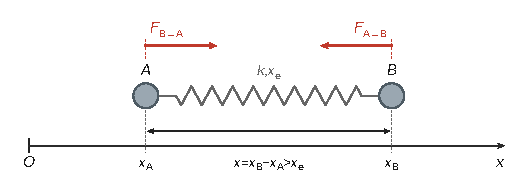
\includegraphics{figures/q07-forces-liaison.pdf}
\caption*{Figure 2 --- Ressort étiré (x \textgreater{} x\_e), la force de B sur A
est dirigée selon +u\_x, celle de A sur B selon −u\_x}
\end{figure}

La deuxième loi de Newton projetée sur \(\vec u_x\) donne \(m_A \ddot x_A = k(x - x_e)\) :

\equationajustee{\boxed{\ddot x_A - \frac{k}{m_A}(x - x_e) = 0}\qquad (2)}

\hypertarget{q8}{%
\subsubsection{Q8}\label{q8}}

Système : atome \(B\), même référentiel.

\equationajustee{\vec F_{A\to B} = -\vec F_{B\to A} = -k(x - x_e)\,\vec u_x}

(troisième loi de Newton ; c'est aussi la loi de Hooke à l'autre extrémité du ressort). D'où \(m_B \ddot x_B = -k(x - x_e)\) :

\equationajustee{\boxed{\ddot x_B + \frac{k}{m_B}(x - x_e) = 0}\qquad (3)}

\textbf{Le signe devant \(k/m_B\) est le signe \(+\).}

\hypertarget{q9}{%
\subsubsection{Q9}\label{q9}}

\equationajustee{\begin{aligned}
\ddot x &= \ddot x_B - \ddot x_A \\
&= -\frac{k}{m_B}(x - x_e) - \frac{k}{m_A}(x - x_e) \\
&= -k\left(\frac{1}{m_A} + \frac{1}{m_B}\right)(x - x_e)
\end{aligned}}

En posant \(\dfrac{1}{\mu} = \dfrac{1}{m_A} + \dfrac{1}{m_B}\) et en multipliant par \(\mu\) : \(\mu \ddot x = -k(x - x_e)\), soit

\equationajustee{\boxed{\begin{aligned}
\mu\ddot x + kx &= kx_e \\
\mu &= \frac{m_A m_B}{m_A + m_B}
\end{aligned}}}

\hypertarget{q10}{%
\subsubsection{Q10}\label{q10}}

Avec \(X = x - x_e\) : \(\ddot X + \dfrac{k}{\mu} X = 0\), oscillateur harmonique de pulsation \(\sqrt{k/\mu}\) :

\equationajustee{\boxed{f_0 = \frac{1}{2\pi}\sqrt{\frac{k}{\mu}}}}

\hypertarget{q11}{%
\subsubsection{Q11}\label{q11}}

Dans le vide \(\lambda_0 = c/f_0\), donc

\equationajustee{\boxed{\sigma_0 = \frac{f_0}{c} = \frac{1}{2\pi c}\sqrt{\frac{k}{\mu}}}}

\hypertarget{validituxe9-de-la-loi-de-hooke-sur-la-multiplicituxe9-de-la-liaison}{%
\subsection{Validité de la loi de Hooke sur la multiplicité de la liaison}\label{validituxe9-de-la-loi-de-hooke-sur-la-multiplicituxe9-de-la-liaison}}

\hypertarget{q12}{%
\subsubsection{Q12}\label{q12}}

Le point de masse \(\mu\), d'abscisse \(x\) comptée depuis le support \(O\), est relié à \(O\) par deux ressorts identiques de longueur \(x\).

Ils ont donc le \textbf{même allongement} \(x - x_e\) et exercent chacun la force \(-k(x - x_e)\vec u_x\). La somme des forces vaut

\equationajustee{\sum \vec F = -2k(x - x_e)\,\vec u_x}

Un ressort unique équivalent exercerait \(-k_{\text{\text{éq}},2}(x - x_e)\,\vec u_x\) ; par identification :

\equationajustee{\boxed{k_{\text{\text{éq}},2} = 2k}}

\hypertarget{q13}{%
\subsubsection{Q13}\label{q13}}

Par le même raisonnement (même allongement pour les trois ressorts, forces qui s'ajoutent) :

\equationajustee{\boxed{k_{\text{\text{éq}},3} = 3k}}

\hypertarget{q14}{%
\subsubsection{Q14}\label{q14}}

La masse réduite est la même (mêmes atomes) ; on remplace \(k\) par la raideur équivalente dans Q11 :

\equationajustee{\boxed{\begin{aligned}
\sigma_{0,2} &= \frac{1}{2\pi c}\sqrt{\frac{2k}{\mu}} \\
&= \sqrt2\,\sigma_0 \\
\sigma_{0,3} &= \frac{1}{2\pi c}\sqrt{\frac{3k}{\mu}} \\
&= \sqrt3\,\sigma_0
\end{aligned}}}

\hypertarget{q15}{%
\subsubsection{Q15}\label{q15}}

Les trois liaisons relient les mêmes atomes C et N, donc \(\mu\) est commun ; le nombre d'onde croît avec la multiplicité (\(\sigma \propto \sqrt{p}\)). On attribue par ordre croissant :

\equationajustee{\boxed{\begin{aligned}
\text{C–N} &: 1{,}30\cdot10^3\ \mathrm{cm^{-1}} \\
\text{C=N} &: 1{,}65\cdot10^3\ \mathrm{cm^{-1}} \\
\text{C}\equiv\text{N} &: 2{,}20\cdot10^3\ \mathrm{cm^{-1}}
\end{aligned}}}

Contrôle : \(\sqrt2 \times 1{,}30\cdot10^3 \approx 1{,}84\cdot10^3\) et \(\sqrt3 \times 1{,}30\cdot10^3 \approx 2{,}25\cdot10^3\ \mathrm{cm^{-1}}\). Le modèle donne le bon ordre ; il surestime la raideur de la double liaison (écart d'environ 11 \%), la triple étant bien décrite (environ 2 \%).

\hypertarget{i.2-moduxe8le-quantique}{%
\subsection{I.2 --- Modèle quantique}\label{i.2-moduxe8le-quantique}}

\hypertarget{q16}{%
\subsubsection{Q16}\label{q16}}

Avec \(\psi(x,t) = \varphi(x)\,{\mathrm{e}}^{-\mathrm{i}Et/\hbar}\) :

\equationajustee{\frac{\partial\psi}{\partial t} = -\frac{\mathrm{i}E}{\hbar}\psi}

\equationajustee{\frac{\partial^2\psi}{\partial x^2} = \varphi''(x)\,{\mathrm{e}}^{-\mathrm{i}Et/\hbar}}

L'équation de Schrödinger donne

\equationajustee{E\varphi(x)\,{\mathrm{e}}^{-\mathrm{i}Et/\hbar} = \left(-\frac{\hbar^2}{2\mu}\varphi''(x) + V(x)\varphi(x)\right){\mathrm{e}}^{-\mathrm{i}Et/\hbar}}

L'exponentielle ne s'annule pas ; on simplifie, et avec \(V = \frac12\mu\omega_0^2 x^2\) :

\equationajustee{\boxed{\frac{{\mathrm{d}}^2\varphi}{\mathrm{d}x^2} + \frac{2\mu}{\hbar^2}\left(E - \tfrac12 \mu\omega_0^2 x^2\right)\varphi(x) = 0}\qquad (6)}

\hypertarget{q17}{%
\subsubsection{Q17}\label{q17}}

Formule de l'annexe appliquée en \(a = x\), avec les accroissements \(+\mathrm{d}x\) et \(-\mathrm{d}x\) :

\equationajustee{\boxed{\varphi(x + \mathrm{d}x) \approx \varphi(x) + \mathrm{d}x\,\varphi'(x) + \frac{\mathrm{d}x^2}{2}\varphi''(x)}}

\equationajustee{\boxed{\varphi(x - \mathrm{d}x) \approx \varphi(x) - \mathrm{d}x\,\varphi'(x) + \frac{\mathrm{d}x^2}{2}\varphi''(x)}}

\hypertarget{q18}{%
\subsubsection{Q18}\label{q18}}

En sommant, les termes d'ordre 1 se compensent :

\equationajustee{\varphi(x+\mathrm{d}x) + \varphi(x - \mathrm{d}x) \approx 2\varphi(x) + \mathrm{d}x^2\,\varphi''(x)}

d'où

\equationajustee{\boxed{\frac{{\mathrm{d}}^2\varphi}{\mathrm{d}x^2} = \frac{\varphi(x + \mathrm{d}x) - 2\varphi(x) + \varphi(x - \mathrm{d}x)}{\mathrm{d}x^2}}}

\hypertarget{q19}{%
\subsubsection{Q19}\label{q19}}

Au point \(x_i\), avec \(\mathrm{d}x = \mathtt{Dx}\), \(x_i \pm \mathtt{Dx} = x_{i\pm1}\) :

\equationajustee{\boxed{\left(\frac{{\mathrm{d}}^2\varphi}{\mathrm{d}x^2}\right)_{x_i} = \frac{\varphi_{i+1} - 2\varphi_i + \varphi_{i-1}}{{\mathtt{Dx}}^2}}}

valable pour \(1 \le i \le N-2\).

\hypertarget{q20}{%
\subsubsection{Q20}\label{q20}}

L'équation (6) en \(x_i\), avec \(E = (n + \frac12)\hbar\omega_0\) et Q19 :

\equationajustee{\begin{aligned}
\varphi_{i+1} - 2\varphi_i + \varphi_{i-1} &= \frac{2\mu}{\hbar^2}\left(\tfrac12\mu\omega_0^2 x_i^2 - (n + \tfrac12)\hbar\omega_0\right){\mathtt{Dx}}^2\,\varphi_i \\
&= \frac{2\mu\omega_0}{\hbar^2}\left(\tfrac12\mu\omega_0 x_i^2 - (n + \tfrac12)\hbar\right){\mathtt{Dx}}^2\,\varphi_i
\end{aligned}}

d'où, en isolant \(\varphi_{i+1}\) et en factorisant 2 :

\equationajustee{\boxed{\varphi_{i+1} = 2\left[1 + \frac{\mu\omega_0}{\hbar^2}\left(\tfrac12\mu\omega_0 x_i^2 - (n + \tfrac12)\hbar\right){\mathtt{Dx}}^2\right]\varphi_i - \varphi_{i-1}}\qquad (7)}

\hypertarget{q21}{%
\subsubsection{Q21}\label{q21}}

\(V(L) = E(5)\) s'écrit \(\frac12\mu\omega_0^2 L^2 = \frac{11}{2}\hbar\omega_0\), d'où (\(L > 0\))

\equationajustee{\boxed{L = \sqrt{\frac{11\hbar}{\mu\omega_0}}}}

AN de contrôle, avec \(\mu\omega_0 = 10^{-14}\) SI :

\equationajustee{\begin{aligned}
L &= \sqrt{11 \times 1{,}05\cdot10^{-34}/10^{-14}} \\
&= \sqrt{1{,}155\cdot10^{-19}} \\
&\approx 3{,}4\cdot10^{-10}\ \mathrm{m}
\end{aligned}}

cohérent avec la figure 7.

\begin{lstlisting}[language=Python]
L = np.sqrt(11 * hbar / (mu * omega0))          # Q21
\end{lstlisting}

\hypertarget{q22}{%
\subsubsection{Q22}\label{q22}}

\begin{lstlisting}[language=Python]
X = np.linspace(-L, L, N)                       # Q22
\end{lstlisting}

\hypertarget{q23}{%
\subsubsection{Q23}\label{q23}}

\(N\) points délimitent \(N - 1\) intervalles sur une longueur \(2L\) :

\begin{lstlisting}[language=Python]
Dx = X[1] - X[0]                                # Q23  (ou Dx = 2 * L / (N - 1))
\end{lstlisting}

\hypertarget{q24}{%
\subsubsection{Q24}\label{q24}}

\begin{lstlisting}[language=Python]
    phi = np.zeros(N)                           # Q24 : phi(x_0) = 0 déjà réalisé
    phi[1] = 1                                  # Q24 : phi(x_1) = 1
\end{lstlisting}

\hypertarget{q25}{%
\subsubsection{Q25}\label{q25}}

La récurrence remplit \(\varphi_{i+1}\) pour \(i\) de 1 à \(N-2\) :

\begin{lstlisting}[language=Python]
    for i in range(1, N - 1):                   # Q25
        phi[i + 1] = 2 * (1 + mu * omega0 / hbar**2 * (0.5 * mu * omega0 * X[i]**2 - (n + 0.5) * hbar) * Dx**2) * phi[i] - phi[i - 1]   # Q25
\end{lstlisting}

(On utilise \texttt{X{[}i{]}} et non \texttt{i*Dx}, puisque \texttt{X} commence à \(-L\).) Le programme complété reproduit la figure 7 (maximum de \(\varphi_0\) voisin de \(7{,}4\cdot10^4\ \mathrm{m^{-1/2}}\)).

\hypertarget{q26}{%
\subsubsection{Q26}\label{q26}}

\(|\varphi(x)|^2\,\mathrm{d}x\) est la probabilité de trouver la particule entre \(x\) et \(x + \mathrm{d}x\). \(K = 1\) est la \textbf{condition de normalisation} : \textbf{la probabilité de trouver la particule dans l'intervalle \([-L, L]\), où elle est localisée, vaut 1 (événement certain).}

\hypertarget{q27}{%
\subsubsection{Q27}\label{q27}}

Méthode des rectangles à gauche sur les \(N-1\) intervalles, de largeur constante \(\mathtt{Dx}\) : \(K \approx \mathtt{Dx}\sum_{i=0}^{N-2}|\varphi_i|^2\).

\begin{lstlisting}[language=Python]
    I = np.sum([abs(phi[i])**2 for i in range(N-1)]) * Dx      # Q27
\end{lstlisting}

La ligne 26 divise alors \texttt{phi} par \(\sqrt{I}\), ce qui rend l'intégrale égale à 1.

\hypertarget{partie-ii-principe-de-fonctionnement-dun-spectrophotomuxe8tre-infrarouge}{%
\section{Partie II --- Principe de fonctionnement d'un spectrophotomètre infrarouge}\label{partie-ii-principe-de-fonctionnement-dun-spectrophotomuxe8tre-infrarouge}}

\hypertarget{ii.1-uxe9tude-de-la-source-infrarouge}{%
\subsection{II.1 --- Étude de la source infrarouge}\label{ii.1-uxe9tude-de-la-source-infrarouge}}

\hypertarget{q28}{%
\subsubsection{Q28}\label{q28}}

\(Z = 28\), règle de Klechkowski :

\equationajustee{\boxed{\mathrm{Ni} : 1s^2\,2s^2\,2p^6\,3s^2\,3p^6\,4s^2\,3d^8 = [\mathrm{Ar}]\,4s^2\,3d^8}}

\(n_{\max} = 4\) : \textbf{4ᵉ période} ; bloc \(d\) avec \(2 + 8 = 10\) électrons de valence (\(4s\) et \(3d\)) : \textbf{groupe 10}.

\hypertarget{q29}{%
\subsubsection{Q29}\label{q29}}

CFC : \(8 \times \frac18 = 1\) atome aux sommets, \(6 \times \frac12 = 3\) aux centres des faces. Les deux centres de faces opposées occupés par Cr comptent \(2 \times \frac12 = 1\) ; il reste \(1 + 4 \times \frac12 = 3\) Ni.

\equationajustee{\boxed{1\ \text{atome de Cr et 3 atomes de Ni par maille (}\mathrm{Ni_3Cr}\text{)}}}

\begin{figure}[H]
\centering
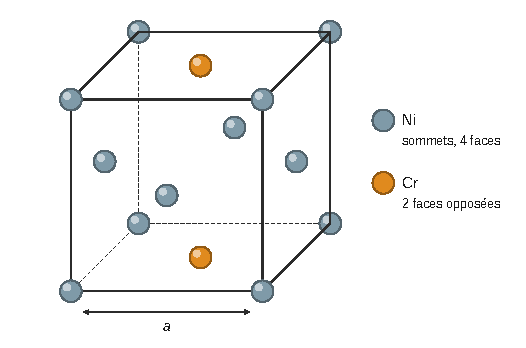
\includegraphics{figures/q29-maille-ni3cr.pdf}
\caption*{Figure 3 --- Maille CFC de l'alliage, Ni aux sommets et sur 4 faces, Cr
au centre de 2 faces opposées}
\end{figure}

\hypertarget{q30}{%
\subsubsection{Q30}\label{q30}}

Masse d'une maille : \(\dfrac{3M_{\mathrm{Ni}} + M_{\mathrm{Cr}}}{N_A}\) ; volume \(a^3\). Donc

\equationajustee{\mu_{\mathrm{NiCr}} = \frac{3M_{\mathrm{Ni}} + M_{\mathrm{Cr}}}{N_A a^3}}

d'où

\equationajustee{\boxed{a = \left(\frac{3M_{\mathrm{Ni}} + M_{\mathrm{Cr}}}{\mu_{\mathrm{NiCr}}\,N_A}\right)^{1/3}}}

\hypertarget{q31}{%
\subsubsection{Q31}\label{q31}}

Dans une structure CFC d'atomes identiques, les plus proches voisins sont un sommet et le centre d'une face adjacente, distants d'une demi-diagonale de face (le contact se fait le long de la diagonale de face) :

\equationajustee{\begin{aligned}
d &= \frac{a\sqrt2}{2} \\
&= \frac{a}{\sqrt2} \\
&= \frac{350}{\sqrt2}\ \mathrm{pm}
\end{aligned}}

\equationajustee{\boxed{d \approx 247\ \mathrm{pm}}}

\hypertarget{q32}{%
\subsubsection{Q32}\label{q32}}

Effet Joule : \(P_{\text{\text{élec}}} = RI^2\) avec \(R = \dfrac{4L}{\gamma\pi D^2}\) :

\equationajustee{\boxed{P_{\text{\text{élec}}} = \frac{4LI^2}{\gamma\pi D^2}}}

\hypertarget{q33}{%
\subsubsection{Q33}\label{q33}}

Surface d'échange : surface latérale \(S = \pi DL\) (extrémités négligées, \(L \gg D\)). Le filament émet \(\sigma T_s^4\) par unité de surface et reçoit \(\sigma T_a^4\) du gaz. Puissance nette cédée par le filament au gaz :

\equationajustee{\boxed{P_{\text{ray}} = \sigma\pi DL\left(T_s^4 - T_a^4\right)}}

\hypertarget{q34}{%
\subsubsection{Q34}\label{q34}}

\equationajustee{\boxed{P_{\text{conv}} = h\pi DL\,(T_s - T_a)}}

comptée elle aussi du filament vers le gaz.

\hypertarget{q35}{%
\subsubsection{Q35}\label{q35}}

En régime permanent (température \(T_s\) atteinte), l'énergie interne du filament est constante : \(P_{\text{\text{élec}}} = P_{\text{ray}} + P_{\text{conv}}\), soit

\equationajustee{\frac{4LI^2}{\gamma\pi D^2} = \pi DL\left[\sigma(T_s^4 - T_a^4) + h(T_s - T_a)\right]}

En divisant par \(\pi DL\) :

\equationajustee{\frac{4I^2}{\gamma\pi^2 D^3} = \sigma T_s^4 - \sigma T_a^4 + hT_s - hT_a}

d'où

\equationajustee{\boxed{\sigma T_a^4 + hT_a = \sigma T_s^4 + hT_s - \frac{4I^2}{\gamma\pi^2 D^3}}\qquad (8)}

\hypertarget{q36}{%
\subsubsection{Q36}\label{q36}}

\(f(T) = \sigma T^4 + hT - \sigma T_s^4 - hT_s + \dfrac{4I^2}{\gamma\pi^2 D^3}\), continue et strictement croissante sur \({\mathbb{R}}^+\). Le code 2 n'importe rien : on ajoute \texttt{from\ math\ import\ pi} en tête du programme.

\begin{lstlisting}[language=Python]
def f(T):
    return sigma * T**4 + h * T - sigma * Ts**4 - h * Ts + 4 * I**2 / (gamma * pi**2 * D**3)   # Q36
\end{lstlisting}

\hypertarget{q37}{%
\subsubsection{Q37}\label{q37}}

\begin{lstlisting}[language=Python]
def dichotomie(f, a, b, eps):                   # Q37
    while b - a > eps:
        m = (a + b) / 2
        if f(m) == 0:
            return m
        if f(a) * f(m) > 0:     # même signe : la racine est dans [m, b]
            a = m
        else:                   # sinon elle est dans [a, m]
            b = m
    return (a + b) / 2
\end{lstlisting}

Invariant : \(f(a)\) et \(f(b)\) sont de signes opposés, la racine est dans \([a, b]\). La largeur est divisée par 2 à chaque tour : de \(702\) K à moins de 1 K en 10 itérations ; le résultat est à moins de \(\varepsilon/2\) de la racine.

\hypertarget{q38}{%
\subsubsection{Q38}\label{q38}}

\(T_a \approx 986\) K est \textbf{inférieure} à \(T_s = 1{,}00\cdot10^3\) K, comme il se doit (le filament chauffe le gaz ; \(f(T_s) > 0\)), et comprise dans l'intervalle de recherche \([298, 1000]\) K. L'écart n'est que d'environ 14 K, soit 1,4 \% de \(T_s\) : le gaz est presque à la température du filament.

Ordres de grandeur :

\equationajustee{\begin{aligned}
\frac{4I^2}{\gamma\pi^2 D^3} &= \frac{4 \times 625}{10^7 \times \pi^2 \times 8\cdot10^{-9}} \\
&\approx 3{,}2\cdot10^3\ \mathrm{W\,m^{-2}}
\end{aligned}}

C'est petit devant \(\sigma T_s^4 = 5{,}67\cdot10^4\ \mathrm{W\,m^{-2}}\) : un faible écart de température suffit à évacuer la puissance Joule.

Le flux conducto-convectif \(h(T_s - T_a) \approx 14\ \mathrm{W\,m^{-2}}\) ne représente que 0,4 \% du total : \textbf{l'échange est presque exclusivement radiatif} car \(h = 1\ \mathrm{W\,m^{-2}\,K^{-1}}\) est très faible.

La valeur est donnée à \(\varepsilon = 1\) K près (trois chiffres significatifs, cohérents avec les données) ; l'écart \(T_s - T_a\) est en revanche très sensible aux données (une variation de 0,5 \% de \(T_s\) déplace \(T_a\) d'environ 5 K). Une température de gaz aussi élevée traduit les limites du modèle (gaz assimilé à un corps noir isotherme, sans autre perte vers les parois).

\hypertarget{ii.2-monochromateur-uxe0-ruxe9seau}{%
\subsection{II.2 --- Monochromateur à réseau}\label{ii.2-monochromateur-uxe0-ruxe9seau}}

\hypertarget{q39}{%
\subsubsection{Q39}\label{q39}}

Repère : \(\vec u_x\) normal au réseau dans le sens de propagation, \(\vec u_y\) le long du réseau dirigé de la fente \(F_2\) (rayon 2) vers la fente \(F_1\) (rayon 1). Les angles sont orientés positivement dans le sens de la figure 9.

Directions incidente et diffractée, et vecteur entre fentes :

\equationajustee{\begin{aligned}
\vec u_i &= \cos i_0\,\vec u_x + \sin i_0\,\vec u_y \\
\vec u_d &= \cos\theta\,\vec u_x + \sin\theta\,\vec u_y \\
\overrightarrow{F_1F_2} &= -a\,\vec u_y
\end{aligned}}

On prend un plan d'onde incident (perpendiculaire à \(\vec u_i\)) et un plan d'onde diffracté (perpendiculaire à \(\vec u_d\)), communs aux deux rayons. Par rapport au rayon (1), le rayon (2) parcourt avant le réseau le chemin supplémentaire \(\vec u_i\cdot\overrightarrow{F_1F_2}\), et après le réseau le chemin supplémentaire \(-\vec u_d\cdot\overrightarrow{F_1F_2}\). Dans l'air (indice 1) :

\equationajustee{\begin{aligned}
\delta_{2/1} &= (\vec u_i - \vec u_d)\cdot\overrightarrow{F_1F_2} \\
&= -a(\sin i_0 - \sin\theta)
\end{aligned}}

\equationajustee{\boxed{\delta_{2/1} = a\left(\sin\theta - \sin i_0\right)}}

\begin{figure}[H]
\centering
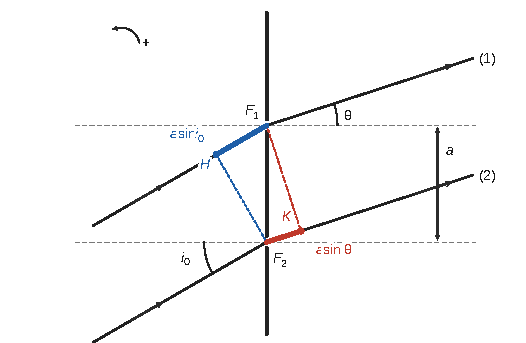
\includegraphics{figures/q39-difference-marche.pdf}
\caption*{Figure 4 --- Plans d'onde par F₂ et par F₁, chemins supplémentaires HF₁
= a sin i₀ et F₂K = a sin θ}
\end{figure}

\hypertarget{q40}{%
\subsubsection{Q40}\label{q40}}

\begin{enumerate}
\def\labelenumi{(\arabic{enumi})}
\setcounter{enumi}{8}
\tightlist
\item
  s'écrit \(a(\sin\theta - \sin i_0) = -\lambda\), soit \(\delta_{2/1} = p\lambda\) avec \(p = -1\).
\end{enumerate}

\textbf{C'est la condition d'interférences constructives entre les ondes issues de toutes les fentes (différence de marche multiple entier de \(\lambda\) entre fentes consécutives) : la direction \(\theta\) est celle d'un maximum principal de diffraction d'ordre \(-1\) pour la longueur d'onde \(\lambda\).}

Cette direction dépend de \(\lambda\) : le réseau disperse la lumière.

\hypertarget{q41}{%
\subsubsection{Q41}\label{q41}}

Les rayons qui convergent au foyer image \(F'\) d'une lentille convergente sont ceux qui arrivent parallèlement à l'axe optique ; la lentille étant parallèle au réseau, son axe est normal au réseau :

\equationajustee{\boxed{\theta = 0}}

Alors (9) donne \(0 = \sin i_0 - \lambda_0/a\) :

\equationajustee{\boxed{i_0 = \arcsin\left(\frac{\lambda_0}{a}\right)}}

qui n'existe que si \(\lambda_0 \le a = 3{,}33\ \mu\)m, soit \(\sigma_0 \ge 3{,}0\cdot10^3\ \mathrm{cm^{-1}}\) (avec ce réseau, la zone 1500--3000 cm⁻¹ étudiée plus loin ne serait pas accessible à l'ordre −1 dans cette configuration : incohérence de données de l'énoncé).

\hypertarget{q42}{%
\subsubsection{Q42}\label{q42}}

Dans les conditions de Gauss, un faisceau parallèle incliné de \(\theta\) sur l'axe converge dans le plan focal image au point d'abscisse \(x = f'\tan\theta \approx f'\theta\). La fente de largeur \(b\), centrée sur \(F'\), a son bord supérieur en \(x = b/2\) :

\equationajustee{\boxed{\theta_\ell = \frac{b}{2f'}}}

AN : \(\theta_\ell = 5\cdot10^{-4}\) rad, angle très petit (conditions de Gauss vérifiées).

\begin{figure}[H]
\centering
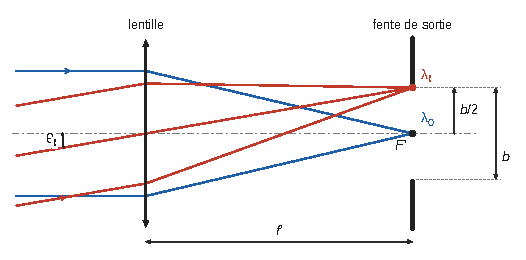
\includegraphics{figures/q42-fente-sortie.pdf}
\caption*{Figure 5 --- Rayons parallèles à l'axe convergeant en F' (λ₀), rayons
inclinés de θ\_ℓ convergeant au bord supérieur de la fente (λ\_ℓ)}
\end{figure}

\hypertarget{q43}{%
\subsubsection{Q43}\label{q43}}

\begin{enumerate}
\def\labelenumi{(\arabic{enumi})}
\setcounter{enumi}{8}
\tightlist
\item
  en \(\theta_\ell\) : \(\lambda_\ell = a(\sin i_0 - \sin\theta_\ell)\), avec \(\sin i_0 = \lambda_0/a\) et \(\sin\theta_\ell \approx \theta_\ell = b/(2f')\) :
\end{enumerate}

\equationajustee{\boxed{\lambda_\ell = \lambda_0 - \frac{ab}{2f'}}}

Le bord inférieur (\(-\theta_\ell\)) correspond à \(\lambda_0 + \dfrac{ab}{2f'}\). Les longueurs d'onde qui atteignent la fente occupent l'intervalle de largeur

\equationajustee{\boxed{\Delta\lambda = \frac{ab}{f'}}}

AN : \(a = \dfrac{1}{3\cdot10^2}\ \mathrm{mm} = 3{,}33\ \mu\mathrm{m}\), \(b = 0{,}1\) mm, \(f' = 100\) mm :

\equationajustee{\Delta\lambda = \frac{3{,}33\cdot10^{-3} \times 0{,}1}{100}\ \mathrm{mm}}

\equationajustee{\boxed{\Delta\lambda \approx 3{,}3\ \mathrm{nm}}}

\textbf{Cette valeur est en bon accord avec la largeur spectrale de 3 nm annoncée par la notice} : la largeur de la fente de sortie suffit à expliquer la résolution du constructeur (la précision et la reproductibilité de ±2 nm relèvent du positionnement du réseau, pas de ce calcul).

\hypertarget{q44}{%
\subsubsection{Q44}\label{q44}}

La transmittance est le rapport de l'intensité transmise par l'échantillon à une intensité de \textbf{référence} (blanc, ligne de base) mesurée séparément. Pour un milieu qui ne fait qu'absorber, \(T \le 100\) \% et \(A \ge 0\). \textbf{Les valeurs \(T > 100\) \% (par exemple 102,2 \% à 1536 cm⁻¹) sont des artefacts de mesure} dans des zones où la solution n'absorbe pas : bruit du détecteur, dérive de la source entre la mesure de référence et celle de l'échantillon, ou absorption parasite (vapeur d'eau, CO₂, solvant, cuve) plus forte lors de la référence que lors de la mesure. L'absorbance vraie y est nulle et le signal fluctue de quelques pour cent autour de 0.

\hypertarget{q45}{%
\subsubsection{Q45}\label{q45}}

\texttt{np.loadtxt} renvoie un tableau à deux dimensions (une ligne par point de mesure, deux colonnes ; la ligne d'en-tête commençant par \texttt{\#} est ignorée).

\begin{itemize}
\tightlist
\item
  Ligne 5 : \texttt{s\ =\ data{[}:,\ 0{]}} extrait la première colonne (toutes les lignes, colonne 0) : tableau des \textbf{nombres d'onde} en \(\mathrm{cm^{-1}}\).
\item
  Ligne 6 : \texttt{T\ =\ data{[}:,\ 1{]}} extrait la seconde colonne : tableau des \textbf{transmittances}, en pourcentage.
\end{itemize}

Les deux tableaux ont la même indexation : \texttt{s{[}i{]}} et \texttt{T{[}i{]}} se rapportent au même point (ce qu'exploite la ligne 19).

\hypertarget{q46}{%
\subsubsection{Q46}\label{q46}}

\(\log\) est le logarithme décimal (\texttt{np.log10} de l'annexe) et \(T\) est donné en pourcentage :

\begin{lstlisting}[language=Python]
A = -np.log10(T / 100)                          # Q46
\end{lstlisting}

\hypertarget{q47}{%
\subsubsection{Q47}\label{q47}}

Un pic est un maximum local strict (\(A_i > A_{i-1}\) et \(A_i > A_{i+1}\)), d'indice \(1 \le i \le n-2\), dont le pourcentage d'absorption atteint le seuil. Avec l'absorbance de Q46, le pourcentage de lumière absorbée vaut \(100(1 - 10^{-A_i}) = 100 - T_i\) (c'est la grandeur tracée sur la figure 11) :

\begin{lstlisting}[language=Python]
    for i in range(1, n - 1):                                                   # Q47
        if A[i] > A[i - 1] and A[i] > A[i + 1] and 100 * (1 - 10**(-A[i])) >= p_abs:   # Q47
            pics.append(i)                                                      # Q47
\end{lstlisting}

Variante équivalente : si l'on stocke à la ligne 7 le pourcentage absorbé \texttt{A\ =\ 100\ -\ T}, le troisième test devient \texttt{A{[}i{]}\ \textgreater{}=\ p\_abs} ; les maxima locaux sont les mêmes (fonctions décroissantes de \(T\)), le tableau d'indices aussi (\texttt{{[}45\ 61\ 103{]}}, soit 2042, 2235 et 2741 cm⁻¹).

\textbf{FIN}

\end{document}
